\begin{frame}[c]
    \frametitle{小型固态近红外光谱仪的设计:概要}
    \begin{itemize}
        \item Zhang, H.;  Wang, X.;  Soos, J.; Crisp, J., Design of a \textcolor{purple}{miniature} solid state \textcolor{red}{NIR} spectrometer. SPIE: 1995; Vol. 2475.
        \item \textcolor{blue}{重要性:}灵敏度高、速度快、无需移动部件、无需机械调整的自校准。
        \item \textcolor{blue}{意义:}可以应用于航空航天领域。
    \end{itemize}
    \begin{figure}[H] %H为当前位置,!htb为忽略美学标准,htbp为浮动图形
        \centering %图片居中
        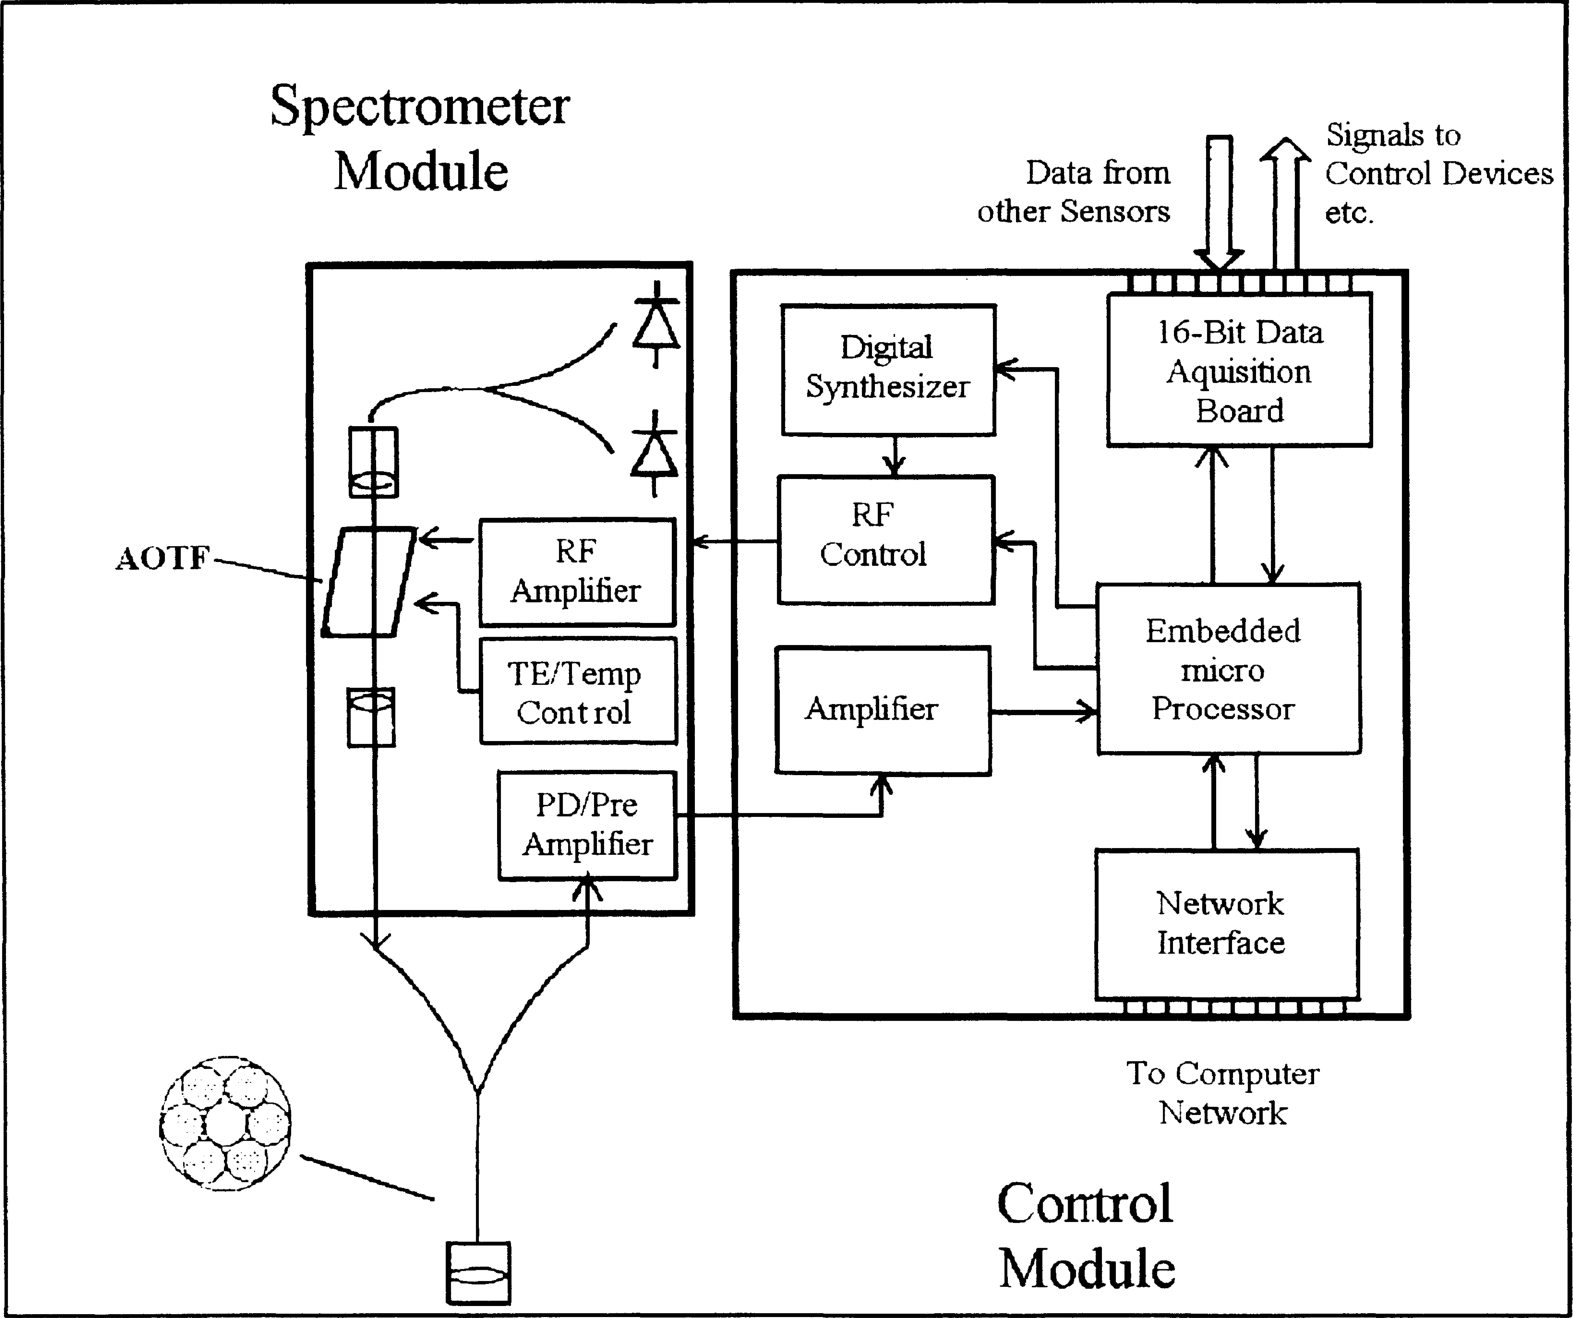
\includegraphics[width=.8\textwidth]{figures/Design of a miniature solid state NIR spectrometer_1.png} %插入图片,[]中设置图片大小,{}中是图片文件名
    \end{figure}
\end{frame}

\begin{frame}[c]
    \frametitle{小型固态近红外光谱仪的设计:原理}
    \begin{enumerate}
        \item 特定频率的信号激励
        \item $\mathrm{TeO}_2$ 晶体中产生声波
        \item 形成周期性的折射率,相当于光子晶体或光栅
        \item 波长满足相位条件的光通过
    \end{enumerate}
    \begin{figure}[H] %H为当前位置,!htb为忽略美学标准,htbp为浮动图形
        \centering %图片居中
        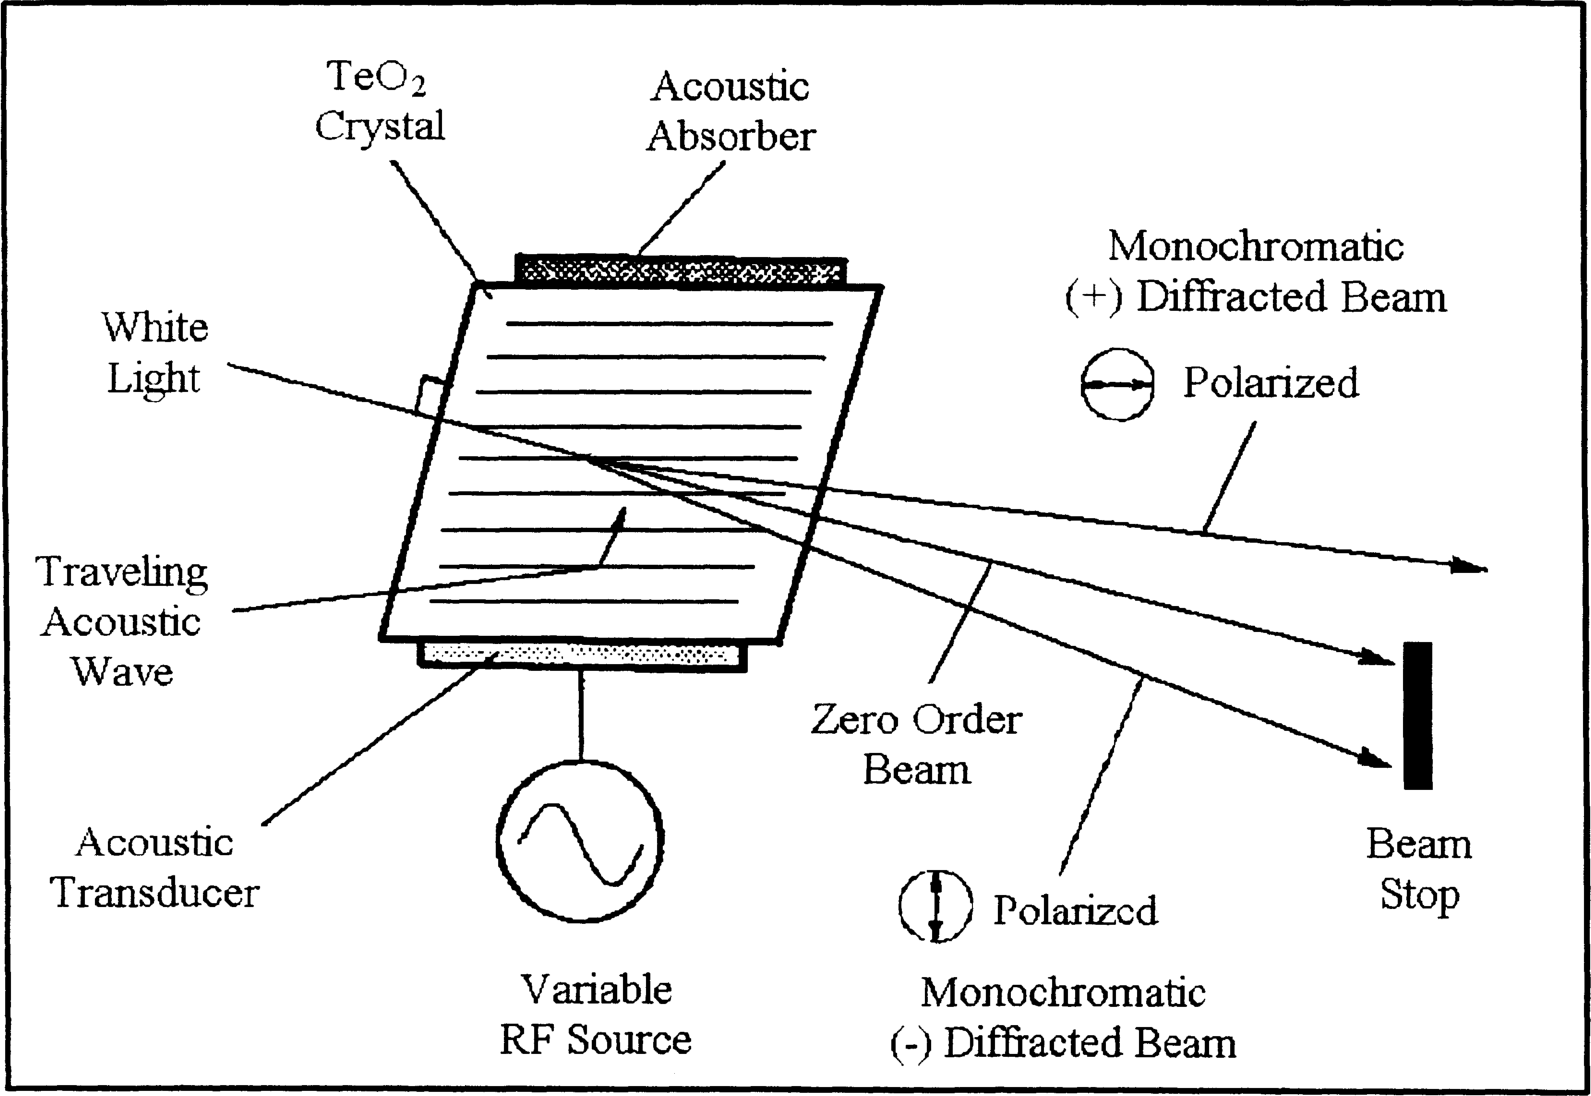
\includegraphics[width=.8\textwidth]{figures/Design of a miniature solid state NIR spectrometer_3.png} %插入图片,[]中设置图片大小,{}中是图片文件名
    \end{figure}
\end{frame}

\begin{frame}[c]
    \frametitle{小型固态近红外光谱仪的设计:实验细节}
    \begin{columns}
        \begin{column}{.4\textwidth}
            LED 代替卤钨灯作光源:
            \begin{itemize}
                \item 节能
                \item 亮度高
                \item 寿命长
                \item 带宽窄
                \item 发光面积小
                \item 稳定
            \end{itemize}
        \end{column}
        \begin{column}{.6\textwidth}
            \begin{figure}[H] %H为当前位置,!htb为忽略美学标准,htbp为浮动图形
                \centering %图片居中
                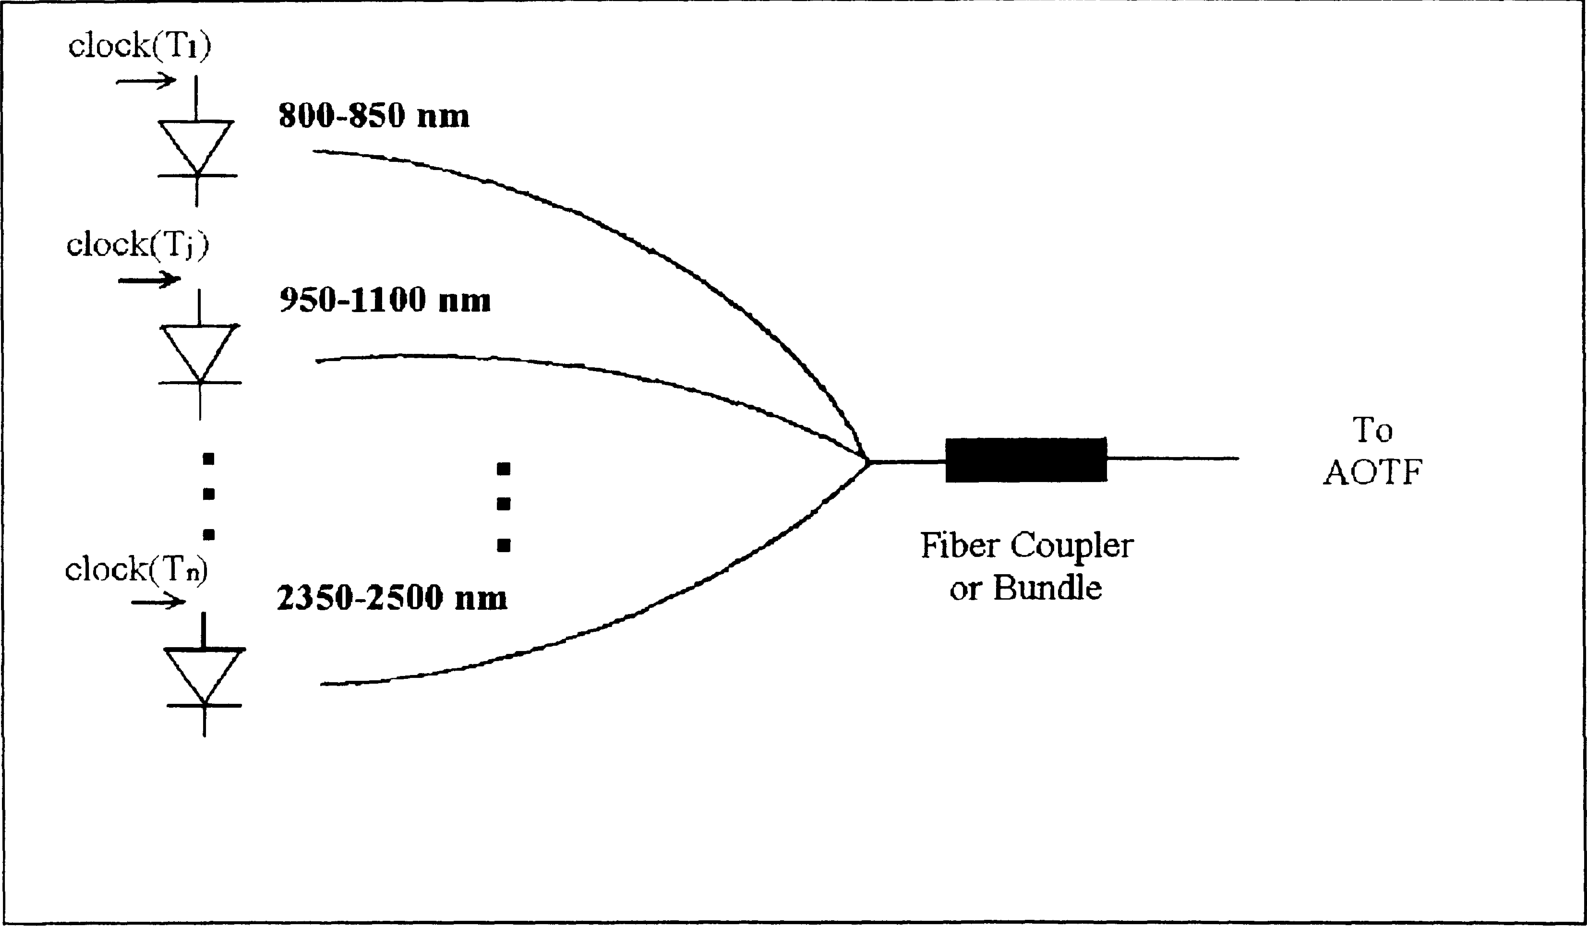
\includegraphics[width=1.\textwidth]{figures/Design of a miniature solid state NIR spectrometer_2.png} %插入图片,[]中设置图片大小,{}中是图片文件名
            \end{figure}
        \end{column}
    \end{columns}
\end{frame}